\subsubsection{Mémoire distribuée}
En mémoire distribuée, nous n'effectuons pas les même calculs qu'en mémoire partagée, mais les accélérations obtenues nous donnerons une approximation des performances que nous pourrons obtenir.
%
Sur la machine Rostand, la factorisation atteint une accélération de 11,8 et la résolution triangulaire une accélération de 3,5.
%
Sur la machine Manumanu, cette accélération monte à pour la factorisation (Fig.~\ref{res_facto_mpi_manu}) et à pour la résolution triangualire (Fig.~\ref{res_trsv_mpi_manu}).


%   (-_-)   %
\begin{figure}[t!]
  \centering
  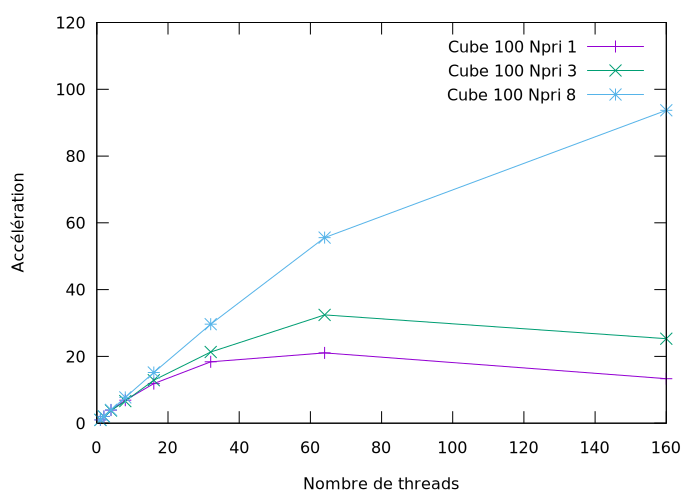
\includegraphics[width=0.7\textwidth]{res_facto_mpi_manu}
  \caption{Performance de la factorisation sur Manumanu en mémoire distribuée.}
  \label{fig:res_facto_mpi_manumanu}
\end{figure}


%   (-_-)   %
\begin{figure}[t!]
  \centering
  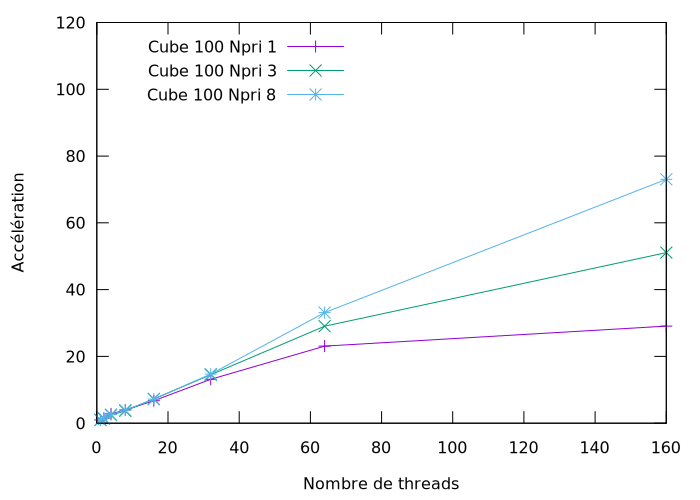
\includegraphics[width=0.7\textwidth]{res_trsv_mpi_manu}
  \caption{Performance de la résolution triangulaire sur Manumanu en mémoire distribuée.}
  \label{fig:res_trsv_mpi_manumanu}
\end{figure}
